%Ukazka zaverecne zpravy
%Posledni zmena 02/2018, Martin Cadik

\documentclass[11pt,a4paper,oneside]{article}
\usepackage[utf8]{inputenc}
\usepackage{a4wide}
\usepackage{url}
\usepackage[breaklinks=true,hidelinks]{hyperref}
%\usepackage[chapter]{algorithm}
%\floatname{algorithm}{Alg.} 
\usepackage{ifpdf}
\ifpdf
\usepackage[pdftex]{graphicx}
\DeclareGraphicsExtensions{.pdf,.png,.gif,.jpg}
\else
\usepackage[final]{graphicx}
\DeclareGraphicsExtensions{.eps,.png,.gif,.jpg}
\fi 
\graphicspath{{fig/}}
\usepackage[export]{adjustbox}


% TODO Jak moc mám přepisovat ten článek.
% TODO jak moc chce popisovat tu implementaci
% TODO uživatelská studie - to mám ukázat metodu lidem a říct mi, která se jim
% líbí víc?

\begin{document}

\thispagestyle{empty}
\begin{center}
\vspace*{60mm}
{Semestrální projekt předmětu Výpočetní fotogragie -- závěrečná zpráva }\\
\smallskip
{\Large\bf Tone Mapping: implementace algoritmu Khan20}\\
\smallskip
{\it Milan Tichavský, \url{xticha09@fit.vut.cz}}\\
\vfill
{\bf Vedoucí práce:} {\it doc. Ing. Martin Čadík, Ph.D., \url{cadik@fit.vut.cz}} 
\hfill {Květen 2025}


\end{center}
\newpage


\section{Úvod}

Zařízení běžně používaná k zobrazování digitálního obsahu, jako jsou monitory,
televizory a tiskárny, nejsou schopna zobrazit celý dynamický rozsah světla
přítomného v reálném světě. Z tohoto důvodu existují metody pro převod obrazu s
vysokým dynamickým rozsahem (HDR) na standardní dynamický rozsah (SDR), aby bylo
možné jej správně vizualizovat na dostupných zařízeních. Tento proces se nazývá
"tone mapping".

Cílem této práce je implementace a analýza jednoho z moderních tone-mapping
algoritmů, konkrétně metody Khan20~\cite{Khan2020}, jako pluginu do Tone Mapping
Studia (TMS)~\cite{TMS2025}.

\section{Teoretické základy}

Pro pochopení tone-mappingu je nutné zmínit vlastnosti lidského vidění. Lidské
oko dokáže adaptivně vnímat velký rozsah jasových hodnot díky nelineárnímu
vnímání jasu a kontrastu. Algoritmy tone-mappingu se často inspirují těmito
vlastnostmi a snaží se přizpůsobit zobrazení tak, aby výsledný obraz působil
přirozeně.

\section{Popis algoritmu Khan20}

Algoritmus Khan20 je globální tone-mapping operator (TMO), to znamená že pro
transformaci je využita monotónní neklesající mapovací funkce. 
Algoritmus je založený na transformaci obrazu pomocí funkce \textit{Perceptual
Quantizer (PQ)} a histogramu jasu. Schéma algoritmu je vidět na obrázku
\ref{fig:schema}.

\begin{figure}[htb]
  \begin{center}
    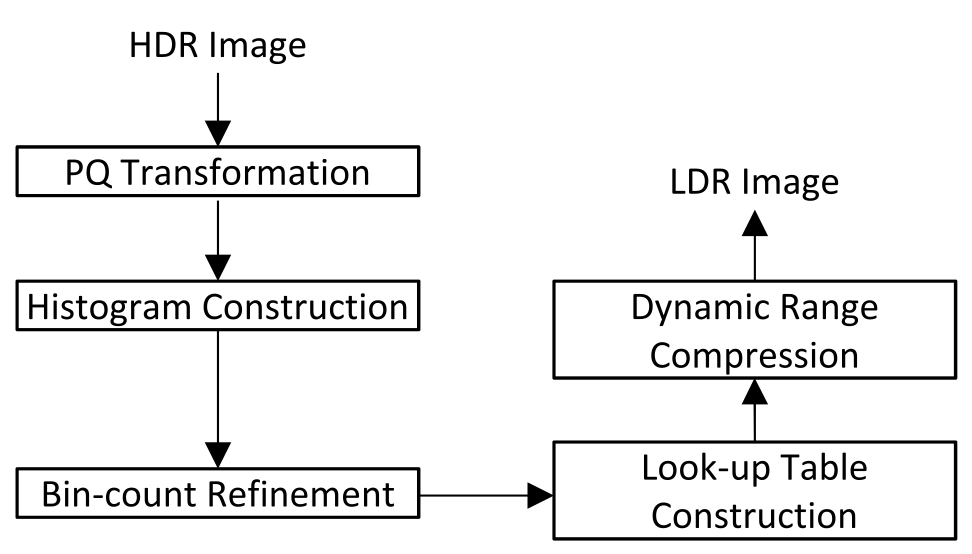
\includegraphics[width=0.8\linewidth]{fig/schema.png}
      \caption{Schéma algoritmu převzato z článku Khan20~\cite{Khan2020}.} 
    \label{fig:schema}
  \end{center}
\end{figure}

Funkce PQ vychází se snaží simulovat vnímaní lidského oka a transformuje
vstupní jas v rozsahu $[0, 10000]$ cd/m$^2$ na normalizovaný rozsah $[0,1]$,
přičemž nižší jasové hodnoty mají k dispozici větší relativní rozlišení.

Jak je vidět v tabulce \ref{tab:method-pq}, z takto transformovaného obrázku lze
jasně vidět celou scénu, která ale působí vybledle a má relativně nízký kontrast.

\begin{table}[htb]
    \centering
    \caption{Obrázky po transformaci funkcí \textit{Perceptual Quantizer}.}
    \label{tab:method-pq}
    \begin{tabular}{lll}
        \includegraphics[width=.33\linewidth,valign=m]{churchKhanPQ.png} &
        \includegraphics[width=.33\linewidth,valign=m]{buildingKhanPQ.png} &
        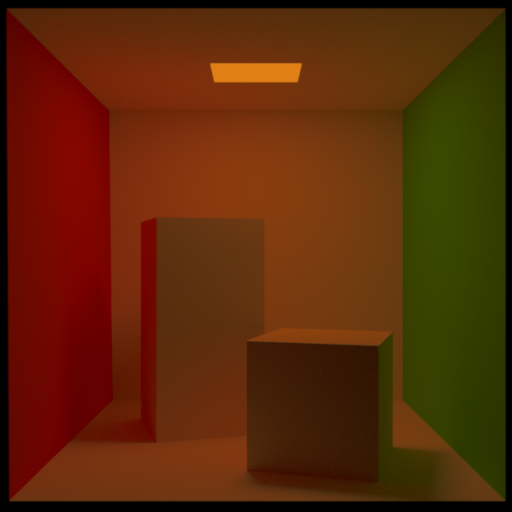
\includegraphics[width=.33\linewidth,valign=m]{cornell_boxKhanPQ.png} \\
    \end{tabular}
\end{table}

The proposed algorithm constructs histogram of
the luminance of the PQ-transformed data, which is used to
design the tone-mapping curve. In addition, a simple and
effective method to handle the issues of excessive enhance-
ment and compression of contrast is proposed. We perform
detailed experimental evaluations using two well-known met-
rics that show a convincingly better performance of the pro-
posed algorithm compared to the existing state of the art
methods


The authors however found that
histogram-based strategy can overly compress some poten-
tially important but smaller regions, and it can be overly
generous to large regions which might not actually need many
display levels. For example, a uniform blue sky covering half
the image certainly does not require half of the total display
levels, which a histogram-based strategy would allocate
The authors of [1] proposed a scheme that tries to solve this
problem by keeping the pixel counts in histogram bins within
defined lower and upper bounds.

Celý postup vypadá následovně:
\begin{itemize}
    \item Transformace HDR obrazu pomocí PQ.
    \item Histogramová úprava kontrastu a binning. % TODO co je binnig
    \item Transformace zpět do SDR.
\end{itemize}

\section{Popis problému a řešení}


Truncation and number of bins.

\subsection{Podsekcí}
Příklad obrázku, viz obr.~\ref{fig:schema}.



\section{Implementace}
Popis implementace a vizualizace jednotlivých fází výpočtu.
\section{Výsledky}

% Nejdůležitější část -- diskuse výsledků, 
% načtené/vypozorované klady a zápory, operační složitost, ...
% Ukázkové obrázky.

See table \ref{tab:method-comp} for comparison agains different methods.
As it can be seen, on all testing images, the scene and all details are very
clearly visible. I think the colors are sometimes bit too light and for more
subjectively better looking images I'd stick with Drago03, as I like the darker and maybe a bit more saturated look of them.
On the other hand, in terms of showing the details in darker regions I think this method is
better.
Also, I really like I don't have to tune parameters of the algorithm for each
scene, because the defaults work across different scenes just fine.

\begin{table}[h]
    \centering
    \caption{Comparison of different methods; first column is Khan20, second
    column Drago03 and third Ward94. All with default values of parameters that
    are set in Tone Mapping Studio.}
    \label{tab:method-comp}
    \begin{tabular}{lll}
        \includegraphics[width=.3\linewidth,valign=m]{churchKhan20.png} &
        \includegraphics[width=.3\linewidth,valign=m]{churchDrago03.png} &
        \includegraphics[width=.3\linewidth,valign=m]{churchWard94.png} \\
    \includegraphics[width=.3\linewidth,valign=m]{buildingKhan20.png} &
        \includegraphics[width=.3\linewidth,valign=m]{buildingDrago03.png} &
        \includegraphics[width=.3\linewidth,valign=m]{buildingWard94.png}\\
    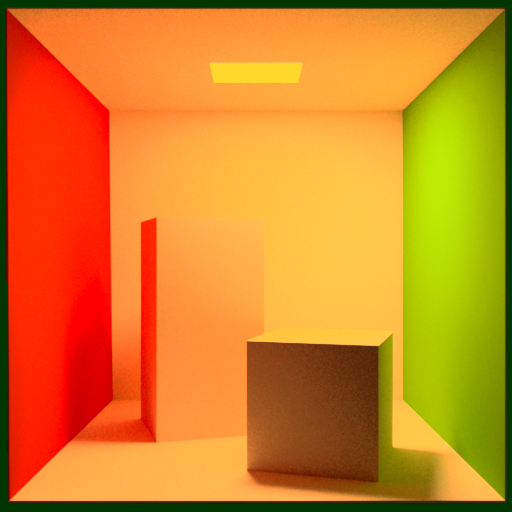
\includegraphics[width=.3\linewidth,valign=m]{cornell_boxKhan20.png} &
        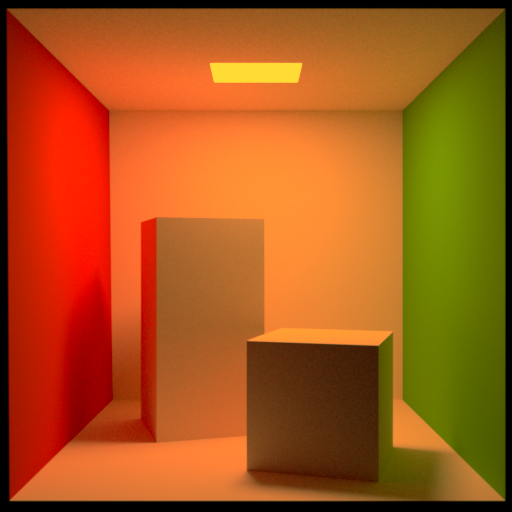
\includegraphics[width=.3\linewidth,valign=m]{cornell_boxDrago03.png} &
        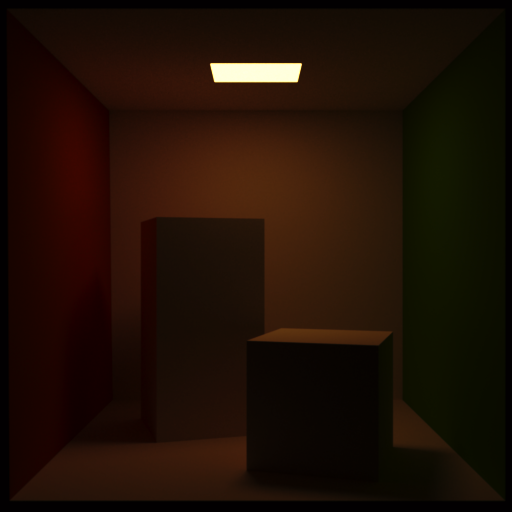
\includegraphics[width=.3\linewidth,valign=m]{cornell_boxWard94.png}\\
    \end{tabular}
\end{table}


Výpočetní složitost implementace je relativně nízká, program projde celkem 4x
přes všechny pixely obrázku a provede relativně jednoduché výpočty v každém
kroku. Počet průchodů by šel snížit, nicméně takto je kód podle mého názoru
přehlednější, kdy se každá funkce mapuje na jednu fázi algoritmu.

\subsection{Uživatelská studie}

Poznatky získané testováním.


\section{Závěr}

\bibliographystyle{acm}
\bibliography{report}

\end{document}
